
\newcommand{\radius}{r}
\newcommand{\dispersion}{d}
\newcommand{\distf}{d}
\newcommand{\dpdim}{\text{dpdim}}
\newcommand{\dpnum}{\text{ep}}

\begin{frame}[fragile]{The doubling constant is a better dimension}

An \textbf{$r$-covering} of a set $X$ is a subset of $X$ such that all pairwise distances are greater than $r$. %$\{x_1,x_2,...x_M\} \subset X$ such that $\dist{x_i}{x_j} > r$ for all distinct $i,j$.

The \textbf{$r$-packing number} $M_r (X)$ is the cardinality of the largest $r$-packing.

The \textbf{doubling constant} of a set $X$ is 
\begin{equation}
\cdoub(X) = \sup_{p\in X,r>0} M_r( B(p,2r))
.
\end{equation}

\vspace{0.15in}
\hrule
\vspace{0.15in}

%The double-packing dimension is defined to be the base 2 logarithm of the double-packing number.
%That is,
%\begin{equation}
%\dpdim(\set X) = \lg \dpnum(\set X)
%.
%\end{equation}
\begin{tabular}{m{4cm}m{7cm} }
\resizebox{!}{3.5cm}{
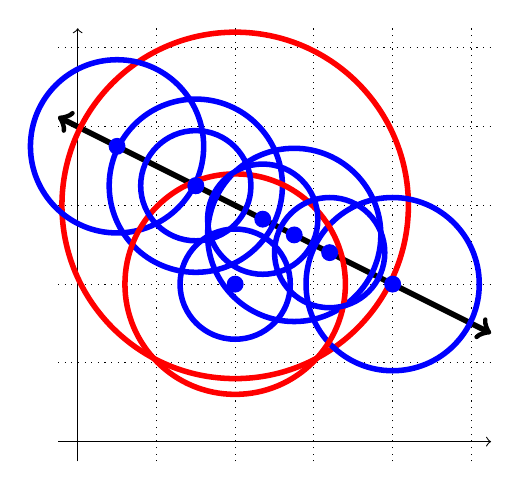
\begin{tikzpicture}[dot/.style={circle,inner sep=2pt,fill,name=#1},
    extended line/.style={shorten >=-#1,shorten <=-#1},
    extended line/.default=1cm]

% draw the grid
\draw[->] (0,-0.25) -- (0,5.25) ;
\draw[->] (-0.25,0) -- (5.25,0) ;
\foreach \i in {1,...,5} {
    \draw[dotted] (-0.25,\i) -- (5.25,\i);
    \draw[dotted] (\i,-0.25) -- (\i,5.25);
}

\draw[line width=2pt,<->] (-0.25,4.125) -- (5.25,1.375);

\uncover<1> {
    %\node at (2.6,3.2) { \textcolor{red}{\Large r} };
    %\path[draw=red,dotted,line width=1pt] (2,3) -- (2.8,3.8);
    \path[draw=red,line width=2pt] (2,3) circle (2.2);

    %\path[draw=red,fill=red] (2,3) circle (0.1);
    %\path[draw=red,line width=2pt] (2,3) circle (1.1);

    \path[draw=blue,fill=blue] (1.5,3.25) circle (0.1);
    \path[draw=blue,line width=2pt] (1.5,3.25) circle (1.1);

    \path[draw=blue,fill=blue] (2.75,2.625) circle (0.1);
    \path[draw=blue,line width=2pt] (2.75,2.625) circle (1.1);

    \path[draw=blue,fill=blue] (4,2) circle (0.1);
    \path[draw=blue,line width=2pt] (4,2) circle (1.1);
    \path[draw=blue,fill=blue] (0.5,3.75) circle (0.1);
    \path[draw=blue,line width=2pt] (0.5,3.75) circle (1.1);
}

\uncover<2> {
    %\node at (2.6,3.2) { \textcolor{red}{\Large r} };
    %\path[draw=red,dotted,line width=1pt] (2,2) -- (2.8,3.8);
    \path[draw=blue,fill=blue] (2,2) circle (0.1);
    \path[draw=blue,line width=2pt] (2,2) circle (0.7);
    \path[draw=red,line width=2pt] (2,2) circle (1.4);

    \path[draw=blue,fill=blue] (1.5,3.25) circle (0.1);
    \path[draw=blue,line width=2pt] (1.5,3.25) circle (0.7);
    \path[draw=blue,fill=blue] (3.2,2.4) circle (0.1);
    \path[draw=blue,line width=2pt] (3.2,2.4) circle (0.7);
    \path[draw=blue,fill=blue] (2.35,2.825) circle (0.1);
    \path[draw=blue,line width=2pt] (2.35,2.825) circle (0.7);
}

%\node[text width=8cm, align=left] at (10,3.5) {
    %\Large
%
%
    %%with the Euclidean distance.
%};


\end{tikzpicture}
}
&
\uncover<1> {
    \textbf{Property 1:}
    Accurately captures the dimension of Euclidean space.
    Specifically,

    \begin{equation}
    \log_2 \dpnum(\mathbb R^n) = O(n)
    \end{equation}

    %In the metric space $\mathbb{R}^n$,
    %$$
    %c
    %= \frac{\pi(2r)^2}{\pi r^2}
    %= 4
    %$$
    %Define the \textbf{expansion-packing dimension} as $\log_2 \dpnum(X)$.
%
    %Then the expansion dimension of $\mathbb{R}^n$ is $O(n)$.
}
\\ &
\vspace{-1.5in}
\uncover<2> {
    \textbf{Property 2:}
    Robust to perturbations in the set $X$.
    For any set $X$ and point $x$, we have that
    \begin{equation}
    \dpnum(X\cup\{x\}) \le \dpnum(X)+1
    \end{equation}
}
%\\ &
%\vspace{-1.75in}
%\uncover<3> {
    %\textbf{Example 3:}
    %In the subspace of $\mathbb{R}^2$ given by
    %$$
    %%\mathcal{X} = \{ (x,y) : y = -0.5x+4 \}
    %\{ (x,y) : y = -0.5x+4 \} \cup \{(2,2)\}
    %$$
    %we have
    %$
    %c
    %%= \frac{\infty}{0}
    %= \infty
    %$
    %%so the expansion dimension is also $\infty$.
%}
\end{tabular}
\end{frame}

